\documentclass[11pt]{article}

\usepackage[margin=1in]{geometry}
\usepackage{hyperref}
\usepackage{fancyhdr}
\usepackage{booktabs}
\usepackage{amsmath}
\usepackage{amssymb}
\usepackage{graphicx}
\usepackage{subcaption}
\usepackage{array}
\usepackage{xcolor}
\usepackage{microtype}

\graphicspath{{../../artifacts/}}
\setlength{\headheight}{14pt}
\newcommand{\fullpageimage}[1]{\includegraphics[width=\textwidth,height=0.82\textheight,keepaspectratio]{#1}}
\newcommand{\largepageimage}[1]{\includegraphics[width=\textwidth,height=0.74\textheight,keepaspectratio]{#1}}

\fancypagestyle{firstpage}{%
  \lhead{NYU Shanghai}
  \rhead{Machine Learning Final Report}
}

\title{Spectral Diagnosis of Inductive Bias in FNO and U-Net for PDEBench 2D CFD}
\author{\href{mailto:wg2139@nyu.edu}{Wenlan Gu}}
\date{\vspace{-5ex}}

\begin{document}
\maketitle
\thispagestyle{firstpage}

\begin{abstract}
This report asks whether the performance of Fourier Neural Operators (FNO) and U-Net on PDEBench 2D compressible CFD can be explained by architectural inductive bias rather than by a single aggregate error score. We evaluate the official PDEBench checkpoints on three regimes that move from smooth low-Mach flow to inviscid shock formation, save full autoregressive validation rollouts, and analyze both models with a redesigned FFT diagnostic. The central methodological change is to replace PDEBench's coarse three-number Fourier metric with normalized radial spectra, bandwise frequency-normalized RMSE, and matched target-vs-prediction contact sheets. The results are strongly regime dependent: FNO's global low-frequency prior is highly effective in the smooth regime, still useful but less dominant in the transitional regime, and much less aligned with the shock regime, where both models approach a representational ceiling. U-Net is consistently worse, especially at high frequency, but the comparison also shows that FNO's advantage is not universal; it depends on whether the physics itself is compatible with a truncated spectral representation.
\end{abstract}

\section{Introduction}
Neural PDE solvers are often compared with a small set of aggregate metrics such as RMSE or nRMSE. That is useful for ranking models, but it is not enough to answer the question that motivated this project: \emph{why} do different model families succeed or fail on different PDE regimes?

This is an inductive-bias question. FNO builds in a spectral prior by representing spatial interactions through global Fourier modes and truncating that representation to a fixed number of low modes \cite{li2021fourier}. U-Net builds in a locality prior by composing local convolutions, pooling, and skip connections \cite{ronneberger2015unet}. In compressible flow, those priors should matter because the solution family changes qualitatively with Mach number and viscosity: smooth regimes are dominated by low-frequency coherent structure, while shock-forming regimes require localized sharp transitions and substantial high-frequency content.

The goal of this report is therefore not just to say which model wins on PDEBench, but to link model performance back to the architecture's innate design choice. To do that, I reorganize evaluation around scale-resolved evidence: Fourier spectra, per-band normalized error, rollout-step RMSE, and target-vs-prediction figures on matched validation samples. The most important sections are thus \textbf{Methods} and \textbf{Experiments}, where the metrics are defined formally and then used to analyze FNO, U-Net, and their direct comparison.

\section{Related Work}
PDEBench provides the dataset family, pretrained baselines, and reference evaluation pipeline used in this project \cite{takamoto2022pdebench}. Its value for this report is that it keeps the PDE family fixed while varying physical difficulty, which makes it possible to study inductive bias under controlled changes in spectral complexity.

FNO is the natural operator-learning baseline because its architecture is itself a statement about how PDE solutions should be represented: global Fourier modes are the primary carriers of information, and only a fixed set of those modes is learned \cite{li2021fourier}. U-Net is the natural image-space control model because it uses local multiscale convolutions without an explicit global spectral basis \cite{ronneberger2015unet}. The comparison is therefore informative even before any new model is designed.

The interpretation also connects to the broader literature on spectral bias, which shows that neural networks tend to fit lower-frequency structure more easily than higher-frequency structure \cite{rahaman2019spectral}. Finally, rollout stability matters in autoregressive PDE prediction, so we preserve PDEBench's pushforward-trained U-Net setting rather than changing the training objective during evaluation \cite{brandstetter2022message}.

\section{Dataset}
The data comes from PDEBench's 2D compressible Navier-Stokes benchmark \cite{takamoto2022pdebench}. Each sample is a tensor with four physical channels: density, pressure, $V_x$, and $V_y$. During evaluation, each rollout has 21 time steps, with the first 10 used as conditioning frames and the remaining 11 produced autoregressively.

I focus on three regimes that form a progression in spectral difficulty:

\begin{table}[t]
\centering
\small
\begin{tabular}{@{}llp{7.0cm}@{}}
\toprule
\textbf{Regime} & \textbf{Validation size} & \textbf{Interpretation} \\
\midrule
$M=0.1,\ \eta=0.1$ & 1000 & Smooth, diffusion-dominated flow; expected best case for FNO's global low-frequency prior \\
$M=1.0,\ \eta=0.01$ & 1000 & Transitional regime with thinner fronts and more mid/high-frequency content \\
$M=1.0,\ \eta=10^{-8}$ & 100 & Inviscid shock regime; strongest test of discontinuity handling \\
\bottomrule
\end{tabular}
\caption{The three PDEBench regimes used in the report. Because the PDE family and channel structure are fixed across rows, changes in model behavior can be interpreted mainly as changes in response to spectral difficulty.}
\label{tab:regimes}
\end{table}

\section{Methods}
\subsection{Evaluation Setup and Notation}
Let $y^{(n)}_{t,c}(x)$ denote the ground-truth field for validation sample $n$, rollout time $t$, channel $c$, and spatial location $x \in \Omega$, and let $\hat{y}^{(n)}_{t,c}(x)$ denote the model prediction. The error field is
\[
e^{(n)}_{t,c}(x) = \hat{y}^{(n)}_{t,c}(x) - y^{(n)}_{t,c}(x).
\]
All rollout analyses are performed after the 10-step conditioning window, so the diagnostic horizon is $t \in \{10,\dots,20\}$. The FNO and U-Net rollouts are extracted from the official PDEBench checkpoints with the same validation split, the same autoregressive horizon, and the same reduced-resolution evaluation grid. This keeps the comparison focused on architectural bias rather than on different training or sampling conditions.

\subsection{Metrics Tracked for Evaluating Each Model}
This subsection defines every metric tracked during evaluation. The first group comes from PDEBench's official evaluation code; the second group was added specifically for this project.

\paragraph{Spatial RMSE.}
Average magnitude of pointwise rollout error in physical space:
\[
\mathrm{RMSE}_{c,t}
=
\frac{1}{N}\sum_{n=1}^{N}
\sqrt{
\frac{1}{|\Omega|}
\sum_{x \in \Omega}
\left(e^{(n)}_{t,c}(x)\right)^2
}.
\]
In PDEBench, the reported scalar is the mean of this quantity over time and then over channels.

\paragraph{Normalized RMSE (nRMSE).}
RMSE scaled by the RMS magnitude of the true signal, so that errors can be compared across channels and regimes with different amplitudes:
\[
\mathrm{nRMSE}_{c,t}
=
\frac{1}{N}\sum_{n=1}^{N}
\frac{
\sqrt{
\frac{1}{|\Omega|}
\sum_{x \in \Omega}
\left(e^{(n)}_{t,c}(x)\right)^2
}
}{
\sqrt{
\frac{1}{|\Omega|}
\sum_{x \in \Omega}
\left(y^{(n)}_{t,c}(x)\right)^2
}
}.
\]

\paragraph{Conserved-variable summary error (CSV).}
Error in the spatially integrated quantity for each channel, useful for checking whether the model gets the global amount of a field roughly right even if the spatial arrangement is imperfect:
\[
\mathrm{CSV}_{c,t}
=
\sqrt{
\frac{1}{N}
\sum_{n=1}^{N}
\left(
\frac{1}{|\Omega|}\sum_{x \in \Omega}\hat{y}^{(n)}_{t,c}(x)
-
\frac{1}{|\Omega|}\sum_{x \in \Omega}y^{(n)}_{t,c}(x)
\right)^2
}.
\]

\paragraph{Max error.}
Worst pointwise error observed anywhere in the validation batch at a given time and channel:
\[
\mathrm{Max}_{c,t}
=
\max_{n,x}
\left|
e^{(n)}_{t,c}(x)
\right|.
\]

\paragraph{Boundary error (BD).}
RMS error restricted to the spatial boundary, used by PDEBench as a diagnostic for boundary degradation. For 2D grids with height $H$ and width $W$:
\[
\mathrm{BD}_{c,t}
=
\frac{1}{N}\sum_{n=1}^{N}
\sqrt{
\frac{1}{2H+2W}
\sum_{x \in \partial \Omega}
\left(e^{(n)}_{t,c}(x)\right)^2
}.
\]

\paragraph{Legacy three-band Fourier error.}
PDEBench's built-in low/mid/high Fourier summary. It is useful as a baseline sanity check, but too coarse for inductive-bias analysis because it averages over time and channel, uses raw shell cutoffs, and does not normalize by the target spectrum. If $E_{\mathrm{err}}(k)$ is the shell-summed error energy at shell index $k$, PDEBench reports
\begin{align}
\mathrm{LegacyLow} &=
\sqrt{\frac{1}{|B_{\mathrm{low}}|}\sum_{k \in B_{\mathrm{low}}} E_{\mathrm{err}}(k)}, \\
\mathrm{LegacyMid} &=
\sqrt{\frac{1}{|B_{\mathrm{mid}}|}\sum_{k \in B_{\mathrm{mid}}} E_{\mathrm{err}}(k)}, \\
\mathrm{LegacyHigh} &=
\sqrt{\frac{1}{|B_{\mathrm{high}}|}\sum_{k \in B_{\mathrm{high}}} E_{\mathrm{err}}(k)}.
\end{align}
with raw shell bands $B_{\mathrm{low}}=[0,4)$, $B_{\mathrm{mid}}=[4,12)$, and $B_{\mathrm{high}}=[12,k_{\max}]$.

\paragraph{Per-step sample RMSE.}
RMSE used in the rollout plots for a specific validation sample at a specific rollout step:
\[
\mathrm{StepRMSE}_{n,t}
=
\sqrt{
\frac{1}{|\Omega|C}
\sum_{c=1}^{C}\sum_{x \in \Omega}
\left(e^{(n)}_{t,c}(x)\right)^2
}.
\]
This metric is not averaged over the whole validation set. It is used to show whether one model stays stable on individual autoregressive sequences.

\subsection{Metrics Designed for Model Comparison}
The central new metrics are designed to answer a different question: not just ``how large is the error,'' but ``how large is the error relative to the amount of true signal in a given frequency range, and how does that differ between models?''

\paragraph{Radial error spectrum and target spectrum.}
Shell-summed Fourier energy of the error and of the ground truth. Let $\mathcal{F}$ denote the 2D FFT over the spatial axes only. For radial shell $k$:
\begin{align}
E^{(n,c,t)}_{\mathrm{err}}(k)
&=
\sum_{\kappa \in \mathrm{shell}(k)}
\left|
\mathcal{F}(e^{(n)}_{t,c})(\kappa)
\right|^2, \\
E^{(n,c,t)}_{\mathrm{target}}(k)
&=
\sum_{\kappa \in \mathrm{shell}(k)}
\left|
\mathcal{F}(y^{(n)}_{t,c})(\kappa)
\right|^2.
\end{align}

\paragraph{Normalized radial coordinate.}
Shell index expressed as a fraction of the Nyquist frequency, so the band definitions are comparable across the reduced $128^2$ and $512^2$ regimes:
\[
\rho = \frac{k}{k_{\mathrm{Nyquist}}}, \qquad \rho \in [0,1].
\]
The three analysis bands are
\[
B_{\mathrm{low}} = [0,1/6), \qquad
B_{\mathrm{mid}} = [1/6,1/3), \qquad
B_{\mathrm{high}} = [1/3,1].
\]

\paragraph{Bandwise frequency-normalized RMSE (fRMSE).}
Error size in a frequency band divided by the signal size in the same band:
\[
\mathrm{fRMSE}^{(n,c,t)}(B)
=
\frac{
\sqrt{\sum_{k \in B} E^{(n,c,t)}_{\mathrm{err}}(k)}
}{
\sqrt{\sum_{k \in B} E^{(n,c,t)}_{\mathrm{target}}(k)} + \varepsilon
}.
\]
If $\mathrm{fRMSE}(B) < 1$, the model's error in band $B$ is smaller than the target signal energy in that band; if it is near or above $1$, the prediction is no longer reliably capturing that scale.

\paragraph{Headline mean band score.}
Validation-set mean of bandwise fRMSE, which is exactly what is stored in each FFT folder's \texttt{headline.csv}:
\[
\overline{\mathrm{fRMSE}}(B)
=
\frac{1}{NCT}
\sum_{n=1}^{N}\sum_{c=1}^{C}\sum_{t}
\mathrm{fRMSE}^{(n,c,t)}(B).
\]
These are the low/mid/high numbers used in the main quantitative tables.

\paragraph{Raw-shell reproduction score.}
Compatibility metric used to check whether the new offline FFT pipeline roughly reproduces PDEBench's legacy three-band output:
\[
\overline{\mathrm{RawShell}}(B)
=
\frac{1}{NCT}
\sum_{n,c,t}
\sqrt{
\frac{1}{|B|}
\sum_{k \in B}
E^{(n,c,t)}_{\mathrm{err}}(k)
}.
\]
This is not the main comparison metric; it is a sanity check against the baseline evaluator.

\paragraph{Model-comparison advantage ratio.}
How many times larger U-Net's bandwise error is than FNO's bandwise error:
\[
A(B)
=
\frac{
\overline{\mathrm{fRMSE}}_{\mathrm{U\text{-}Net}}(B)
}{
\overline{\mathrm{fRMSE}}_{\mathrm{FNO}}(B)
}.
\]
This ratio is the cleanest summary of model comparison because it maps directly onto the inductive-bias question: it says where FNO's spectral prior helps, where it stops helping, and where both models are similarly limited.

\section{Experiments}
\subsection{FNO Performance Analysis}
Table~\ref{tab:fno-metrics} summarizes the FNO FFT results recorded in the three \texttt{artifacts/fno\_fft/.../headline.csv} files. Two patterns are immediate. First, the smooth regime is FNO's best case: low-band $\overline{\mathrm{fRMSE}}$ is still above 1 because the band is normalized by target energy, but the absolute raw-shell numbers are extremely small. Second, the shock regime is qualitatively different: all three fRMSE bands are close to 1, which means the model error has grown to the same order as the signal itself across much of the spectrum.

\begin{table}[t]
\centering
\small
\begin{tabular}{@{}lccc|ccc@{}}
\toprule
\textbf{Regime} & \multicolumn{3}{c|}{\(\overline{\mathrm{fRMSE}}\)} & \multicolumn{3}{c}{\(\overline{\mathrm{RawShell}}\)} \\
 & Low & Mid & High & Low & Mid & High \\
\midrule
Smooth & 1.221 & 48.734 & 397.673 & 0.00501 & 0.00158 & 0.00032 \\
Transitional & 0.208 & 3.033 & 13.747 & 0.14097 & 0.06078 & 0.01320 \\
Shock & 0.675 & 1.029 & 1.023 & 0.99988 & 0.33586 & 0.04845 \\
\bottomrule
\end{tabular}
\caption{FNO headline FFT metrics from the three \texttt{fno\_fft} folders. The fRMSE columns are the main diagnostic; the raw-shell columns are included as baseline-reproduction checks.}
\label{tab:fno-metrics}
\end{table}

\begin{figure}[p]
\centering
\begin{subfigure}[t]{0.32\linewidth}
    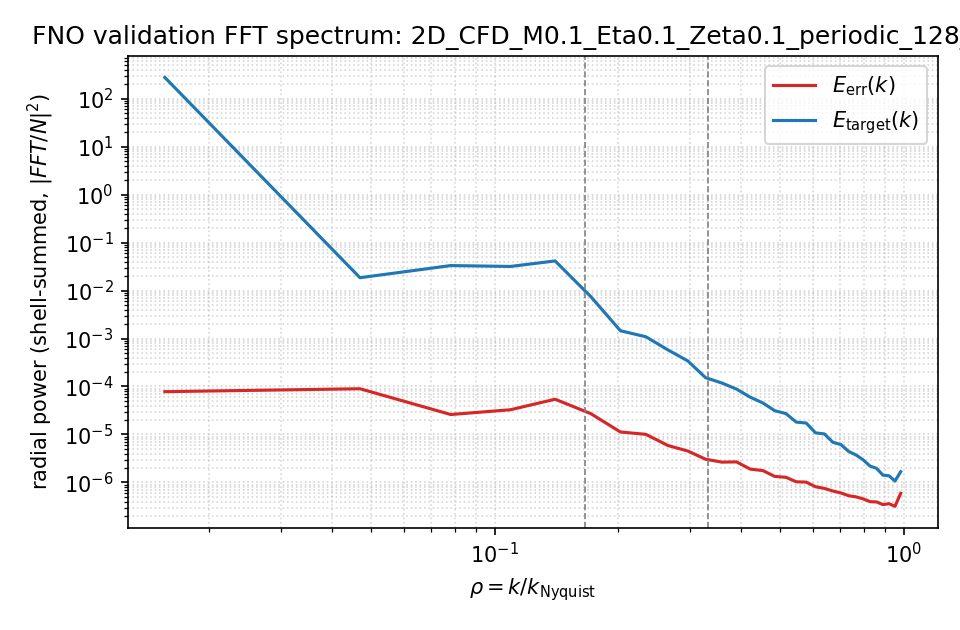
\includegraphics[width=\linewidth]{fno_fft/2D_CFD_M0.1_Eta0.1_Zeta0.1_periodic_128_Train/fft_error_spectrum.png}
    \caption{Smooth regime}
\end{subfigure}\hfill
\begin{subfigure}[t]{0.32\linewidth}
    
\includegraphics[width=\linewidth]{fno_fft/2D_CFD_M1.0_Eta0.01_Zeta0.01_periodic_128_Train/fft_error_spectrum.png}
    \caption{Transitional regime}
\end{subfigure}\hfill
\begin{subfigure}[t]{0.32\linewidth}
    
\includegraphics[width=\linewidth]{fno_fft/2D_CFD_M1.0_Eta1e-08_Zeta1e-08_periodic_512_Train/fft_error_spectrum.png}
    \caption{Shock regime}
\end{subfigure}
\caption{Radial FFT error of FNO in the smooth, transitional, and shock regimes. In each panel, the blue curve denotes the mean target spectrum, the red curve denotes the mean error spectrum, and the dashed vertical lines mark the band boundaries at \(\rho=1/6\) and \(\rho=1/3\).}
\label{fig:fno-fft}
\end{figure}

\paragraph{FNO analysis by regime.}
\textbf{Smooth regime.} FNO is strongest when the solution is globally coherent and low-frequency dominated. Figure~\ref{fig:fno-fft} shows a large gap between target and error spectra across the three bands, and the representative rollout visualizations in Appendix Figures~\ref{fig:app-fno-contact-smooth}--\ref{fig:app-fno-contact-shock} show close agreement with the target in the smooth case. The headline raw-shell errors are extremely small, which is consistent with that visual match. \\
\textbf{Transitional regime.} FNO still resolves the dominant fronts, but the spectral gap narrows, especially in the mid and high bands. The mean scores \((0.208,\,3.033,\,13.747)\) show that FNO still has an advantage but no longer fits the full signal comfortably outside the low band. The transitional appendix visualizations show that front locations are preserved better than fine-scale pressure detail. \\
\textbf{Shock regime.} FNO no longer behaves like a model with a strong margin over the target spectrum. The mean scores \((0.675,\,1.029,\,1.023)\) indicate that, on average, the error is of the same order as the target signal in the mid and high bands. This is consistent with the architectural interpretation that a truncated global Fourier basis is not naturally suited to discontinuities.

\subsection{U-Net Performance Analysis}
Table~\ref{tab:unet-metrics} gives the corresponding U-Net results from the three \texttt{artifacts/unet\_fft/.../headline.csv} files. Across all regimes, U-Net is worse than FNO in every band, but the way it is worse is itself informative. The smooth regime is catastrophic in relative spectral terms, with extremely large mid/high fRMSE. The shock regime remains difficult as well, but the most persistent weakness is high-frequency resolution rather than low-frequency tracking.

\begin{table}[t]
\centering
\small
\begin{tabular}{@{}lccc|ccc@{}}
\toprule
\textbf{Regime} & \multicolumn{3}{c|}{\(\overline{\mathrm{fRMSE}}\)} & \multicolumn{3}{c}{\(\overline{\mathrm{RawShell}}\)} \\
 & Low & Mid & High & Low & Mid & High \\
\midrule
Smooth & 9.719 & 2076.097 & 119855.805 & 0.04896 & 0.01371 & 0.00872 \\
Transitional & 0.644 & 5.330 & 78.204 & 0.41510 & 0.08244 & 0.02928 \\
Shock & 0.882 & 1.363 & 5.563 & 1.17756 & 0.36907 & 0.05720 \\
\bottomrule
\end{tabular}
\caption{U-Net headline FFT metrics from the three \texttt{unet\_fft} folders. The same interpretation as Table~\ref{tab:fno-metrics} applies.}
\label{tab:unet-metrics}
\end{table}

\begin{figure}[p]
\centering
\begin{subfigure}[t]{0.32\linewidth}
    
\includegraphics[width=\linewidth]{unet_fft/2D_CFD_M0.1_Eta0.1_Zeta0.1_periodic_128_Train/fft_error_spectrum.png}
    \caption{Smooth regime}
\end{subfigure}\hfill
\begin{subfigure}[t]{0.32\linewidth}
    
\includegraphics[width=\linewidth]{unet_fft/2D_CFD_M1.0_Eta0.01_Zeta0.01_periodic_128_Train/fft_error_spectrum.png}
    \caption{Transitional regime}
\end{subfigure}\hfill
\begin{subfigure}[t]{0.32\linewidth}
    
\includegraphics[width=\linewidth]{unet_fft/2D_CFD_M1.0_Eta1e-08_Zeta1e-08_periodic_512_Train/fft_error_spectrum.png}
    \caption{Shock regime}
\end{subfigure}
\caption{Radial FFT error of U-Net in the smooth, transitional, and shock regimes. In each panel, the blue curve denotes the mean target spectrum, the red curve denotes the mean error spectrum, and the dashed vertical lines mark the band boundaries at \(\rho=1/6\) and \(\rho=1/3\).}
\label{fig:unet-fft}
\end{figure}

\paragraph{U-Net analysis by regime.}
\textbf{Smooth regime.} U-Net performs especially poorly when the flow is globally smooth. This is not because the task is hard; it is because locality alone is the wrong inductive bias for a globally coherent low-frequency field. The smooth-regime fRMSE values \((9.719,\,2076.097,\,119855.805)\) show that U-Net misses not only fine detail but also a large fraction of the meaningful spectral content outside the very lowest band. Appendix Figures~\ref{fig:app-unet-contact-smooth}--\ref{fig:app-unet-contact-shock} show that this manifests visually as substantial smoothing and loss of contrast. \\
\textbf{Transitional regime.} U-Net becomes more competitive at the lowest frequencies, but it still under-resolves the sharper structure that defines the regime. The appendix visualizations show that the coarse front position is often approximately right, but the predicted field is too smooth and too low-contrast. \\
\textbf{Shock regime.} U-Net captures the broad shock envelope somewhat better than it captures the delicate pressure geometry around it, but its high-band mean score remains \(5.563\), far larger than FNO's \(1.023\). This suggests that U-Net's locality prior is not enough to prevent severe sharpening loss during autoregressive rollout.

\subsection{Model Comparison}
Table~\ref{tab:ratio} gives the most compact cross-model summary: the bandwise U-Net/FNO advantage ratio \(A(B)\). Ratios much larger than 1 indicate that FNO is substantially better in that band. The table makes the regime dependence explicit. In the smooth regime, FNO is overwhelmingly better everywhere. In the transitional regime, the gap narrows, especially in the mid band. In the shock regime, the low- and mid-band gaps nearly collapse, but the high-band gap remains large.

\begin{table}[t]
\centering
\small
\begin{tabular}{@{}lccc@{}}
\toprule
\textbf{Regime} & \textbf{Low} & \textbf{Mid} & \textbf{High} \\
\midrule
Smooth & $7.96\times$ & $42.60\times$ & $301.39\times$ \\
Transitional & $3.09\times$ & $1.76\times$ & $5.69\times$ \\
Shock & $1.31\times$ & $1.32\times$ & $5.44\times$ \\
\bottomrule
\end{tabular}
\caption{Bandwise U-Net/FNO advantage ratio \(A(B)\). Values above 1 mean FNO has lower mean bandwise fRMSE.}
\label{tab:ratio}
\end{table}

\begin{figure}[p]
\centering
\begin{subfigure}[t]{0.48\linewidth}
    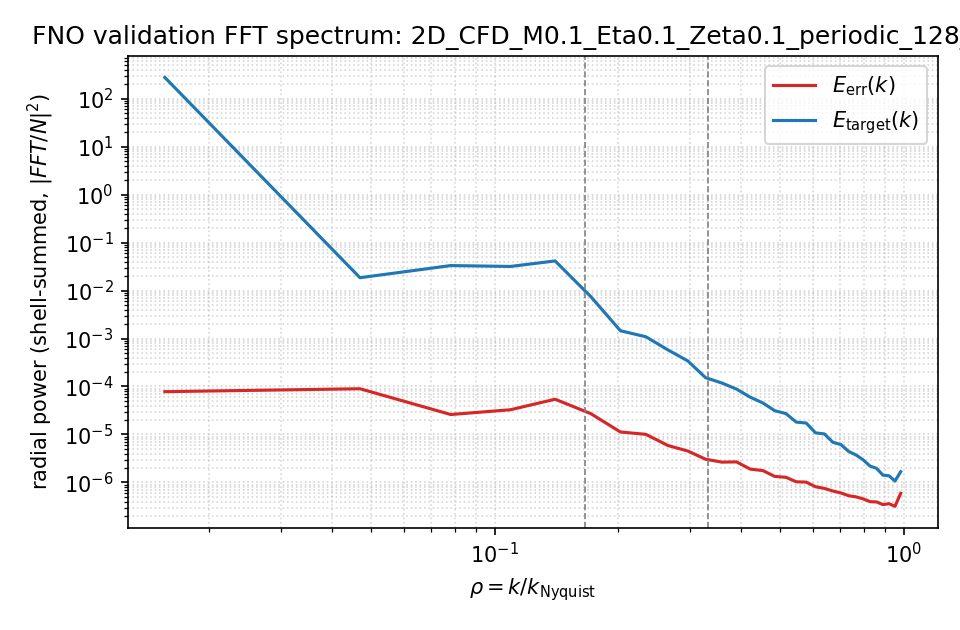
\includegraphics[width=\linewidth]{fno_fft/2D_CFD_M0.1_Eta0.1_Zeta0.1_periodic_128_Train/fft_error_spectrum.png}
    \caption{FNO, smooth}
\end{subfigure}\hfill
\begin{subfigure}[t]{0.48\linewidth}
    
\includegraphics[width=\linewidth]{unet_fft/2D_CFD_M0.1_Eta0.1_Zeta0.1_periodic_128_Train/fft_error_spectrum.png}
    \caption{U-Net, smooth}
\end{subfigure}

\medskip

\begin{subfigure}[t]{0.48\linewidth}
    
\includegraphics[width=\linewidth]{fno_fft/2D_CFD_M1.0_Eta0.01_Zeta0.01_periodic_128_Train/fft_error_spectrum.png}
    \caption{FNO, transitional}
\end{subfigure}\hfill
\begin{subfigure}[t]{0.48\linewidth}
    
\includegraphics[width=\linewidth]{unet_fft/2D_CFD_M1.0_Eta0.01_Zeta0.01_periodic_128_Train/fft_error_spectrum.png}
    \caption{U-Net, transitional}
\end{subfigure}

\medskip

\begin{subfigure}[t]{0.48\linewidth}
    
\includegraphics[width=\linewidth]{fno_fft/2D_CFD_M1.0_Eta1e-08_Zeta1e-08_periodic_512_Train/fft_error_spectrum.png}
    \caption{FNO, shock}
\end{subfigure}\hfill
\begin{subfigure}[t]{0.48\linewidth}
    
\includegraphics[width=\linewidth]{unet_fft/2D_CFD_M1.0_Eta1e-08_Zeta1e-08_periodic_512_Train/fft_error_spectrum.png}
    \caption{U-Net, shock}
\end{subfigure}
\caption{Direct FFT comparison of FNO and U-Net across all three datasets. Within each regime, the left panel shows FNO and the right panel shows U-Net; blue denotes the mean target spectrum, red denotes the mean error spectrum, and dashed lines mark the radial band boundaries used in the tables.}
\label{fig:compare-fft}
\end{figure}

\paragraph{Comparison summary.}
The comparison section answers the central question of the report. FNO's architectural advantage is real, but it is not uniform. In the smooth regime, FNO's global low-frequency bias is almost perfectly aligned with the physics, so it dominates across all bands. In the transitional regime, the advantage shrinks because the solution now contains sharper, more localized structure that is less compatible with a strongly truncated spectral basis. In the shock regime, the low- and mid-band comparison nearly saturates: both models are now close to the target spectrum itself. The remaining advantage for FNO is concentrated in the high band, where U-Net smooths away even more detail than FNO does. The appendix visualizations and per-step RMSE plots confirm that this conclusion is not driven by a single sample.

This leads to a precise inductive-bias interpretation. FNO succeeds when the PDE solution can be represented efficiently by globally coherent low modes. U-Net succeeds only partially because locality alone is not enough to model long-range coordinated flow, and it pays an additional penalty in high-frequency sharpness during autoregressive rollout. Neither model is naturally ideal for discontinuities. That is why the shock regime looks like a ceiling for both, not a victory for either.

\section{Conclusion}
The most important outcome of this report is methodological: the question ``which model is better?'' was too weak. The more informative question is ``which model prior matches which flow regime, and at which spatial scales?'' Once the analysis is expressed in those terms, the results become coherent.

FNO performs best when the target dynamics are smooth and spectrally concentrated, because its global Fourier parameterization directly matches that regime. U-Net performs worse across all regimes, especially at mid and high frequencies, because its locality prior promotes blur and weak long-range coordination. But the comparison also shows that FNO's advantage has clear limits. In the inviscid shock regime, both models approach a regime-level difficulty ceiling, which suggests that future work should combine global operator structure with stronger localized mechanisms for discontinuities instead of relying on either a purely truncated spectral basis or a purely local convolutional hierarchy.

\clearpage
\bibliographystyle{IEEEtran}
\bibliography{references}

\appendix

\section{Additional Rollout Visualizations}

\subsection{Target-vs-FNO Rollouts}
\begin{figure}[p]
\centering
\fullpageimage{figures/model_target_contact/fno/2D_CFD_M0.1_Eta0.1_Zeta0.1_periodic_128_Train/target_vs_pred.png}
\caption{Visualization of the smooth-regime density rollout, comparing ground-truth targets (top row in each sample block) with FNO predictions (bottom row). Columns correspond to rollout steps \(t=10,\dots,20\).}
\label{fig:app-fno-contact-smooth}
\end{figure}

\begin{figure}[p]
\centering
\fullpageimage{figures/model_target_contact/fno/2D_CFD_M1.0_Eta0.01_Zeta0.01_periodic_128_Train/target_vs_pred.png}
\caption{Visualization of the transitional-regime pressure rollout, comparing ground-truth targets with FNO predictions.}
\label{fig:app-fno-contact-transitional}
\end{figure}

\begin{figure}[p]
\centering
\fullpageimage{figures/model_target_contact/fno/2D_CFD_M1.0_Eta1e-08_Zeta1e-08_periodic_512_Train/target_vs_pred.png}
\caption{Visualization of the shock-regime pressure rollout, comparing ground-truth targets with FNO predictions.}
\label{fig:app-fno-contact-shock}
\end{figure}

\subsection{Target-vs-U-Net Rollouts}
\begin{figure}[p]
\centering
\fullpageimage{figures/model_target_contact/unet/2D_CFD_M0.1_Eta0.1_Zeta0.1_periodic_128_Train/target_vs_pred.png}
\caption{Visualization of the smooth-regime density rollout, comparing ground-truth targets (top row in each sample block) with U-Net predictions (bottom row).}
\label{fig:app-unet-contact-smooth}
\end{figure}

\begin{figure}[p]
\centering
\fullpageimage{figures/model_target_contact/unet/2D_CFD_M1.0_Eta0.01_Zeta0.01_periodic_128_Train/target_vs_pred.png}
\caption{Visualization of the transitional-regime pressure rollout, comparing ground-truth targets with U-Net predictions.}
\label{fig:app-unet-contact-transitional}
\end{figure}

\begin{figure}[p]
\centering
\fullpageimage{figures/model_target_contact/unet/2D_CFD_M1.0_Eta1e-08_Zeta1e-08_periodic_512_Train/target_vs_pred.png}
\caption{Visualization of the shock-regime pressure rollout, comparing ground-truth targets with U-Net predictions.}
\label{fig:app-unet-contact-shock}
\end{figure}

\subsection{Channel-wise FNO/U-Net Comparisons}
\begin{figure}[p]
\centering
\fullpageimage{figures/fno_unet_rollout_compare/2D_CFD_M0.1_Eta0.1_Zeta0.1_periodic_128_Train/contact_sheet_density.png}
\caption{Channel-wise comparison for the smooth regime, density channel. Within each sample block, the top row denotes the ground truth, the middle row denotes FNO, and the bottom row denotes U-Net.}
\label{fig:app-compare-density-smooth}
\end{figure}

\begin{figure}[p]
\centering
\fullpageimage{figures/fno_unet_rollout_compare/2D_CFD_M0.1_Eta0.1_Zeta0.1_periodic_128_Train/contact_sheet_pressure.png}
\caption{Channel-wise comparison for the smooth regime, pressure channel.}
\label{fig:app-compare-pressure-smooth}
\end{figure}

\begin{figure}[p]
\centering
\fullpageimage{figures/fno_unet_rollout_compare/2D_CFD_M0.1_Eta0.1_Zeta0.1_periodic_128_Train/contact_sheet_Vx.png}
\caption{Channel-wise comparison for the smooth regime, \(V_x\) channel.}
\label{fig:app-compare-vx-smooth}
\end{figure}

\begin{figure}[p]
\centering
\fullpageimage{figures/fno_unet_rollout_compare/2D_CFD_M0.1_Eta0.1_Zeta0.1_periodic_128_Train/contact_sheet_Vy.png}
\caption{Channel-wise comparison for the smooth regime, \(V_y\) channel.}
\label{fig:app-compare-vy-smooth}
\end{figure}

\begin{figure}[p]
\centering
\fullpageimage{figures/fno_unet_rollout_compare/2D_CFD_M1.0_Eta0.01_Zeta0.01_periodic_128_Train/contact_sheet_density.png}
\caption{Channel-wise comparison for the transitional regime, density channel.}
\label{fig:app-compare-density-transitional}
\end{figure}

\begin{figure}[p]
\centering
\fullpageimage{figures/fno_unet_rollout_compare/2D_CFD_M1.0_Eta0.01_Zeta0.01_periodic_128_Train/contact_sheet_pressure.png}
\caption{Channel-wise comparison for the transitional regime, pressure channel.}
\label{fig:app-compare-pressure-transitional}
\end{figure}

\begin{figure}[p]
\centering
\fullpageimage{figures/fno_unet_rollout_compare/2D_CFD_M1.0_Eta0.01_Zeta0.01_periodic_128_Train/contact_sheet_Vx.png}
\caption{Channel-wise comparison for the transitional regime, \(V_x\) channel.}
\label{fig:app-compare-vx-transitional}
\end{figure}

\begin{figure}[p]
\centering
\fullpageimage{figures/fno_unet_rollout_compare/2D_CFD_M1.0_Eta0.01_Zeta0.01_periodic_128_Train/contact_sheet_Vy.png}
\caption{Channel-wise comparison for the transitional regime, \(V_y\) channel.}
\label{fig:app-compare-vy-transitional}
\end{figure}

\begin{figure}[p]
\centering
\fullpageimage{figures/fno_unet_rollout_compare/2D_CFD_M1.0_Eta1e-08_Zeta1e-08_periodic_512_Train/contact_sheet_density.png}
\caption{Channel-wise comparison for the shock regime, density channel.}
\label{fig:app-compare-density-shock}
\end{figure}

\begin{figure}[p]
\centering
\fullpageimage{figures/fno_unet_rollout_compare/2D_CFD_M1.0_Eta1e-08_Zeta1e-08_periodic_512_Train/contact_sheet_pressure.png}
\caption{Channel-wise comparison for the shock regime, pressure channel.}
\label{fig:app-compare-pressure-shock}
\end{figure}

\begin{figure}[p]
\centering
\fullpageimage{figures/fno_unet_rollout_compare/2D_CFD_M1.0_Eta1e-08_Zeta1e-08_periodic_512_Train/contact_sheet_Vx.png}
\caption{Channel-wise comparison for the shock regime, \(V_x\) channel.}
\label{fig:app-compare-vx-shock}
\end{figure}

\begin{figure}[p]
\centering
\fullpageimage{figures/fno_unet_rollout_compare/2D_CFD_M1.0_Eta1e-08_Zeta1e-08_periodic_512_Train/contact_sheet_Vy.png}
\caption{Channel-wise comparison for the shock regime, \(V_y\) channel.}
\label{fig:app-compare-vy-shock}
\end{figure}

\subsection{Per-step Sample RMSE}
\begin{figure}[p]
\centering
\largepageimage{figures/fno_unet_rollout_compare/2D_CFD_M0.1_Eta0.1_Zeta0.1_periodic_128_Train/rmse_5samples_per_timestep.png}
\caption{Per-step sample RMSE for the smooth regime. Blue denotes FNO and orange denotes U-Net.}
\label{fig:app-rmse-smooth}
\end{figure}

\begin{figure}[p]
\centering
\largepageimage{figures/fno_unet_rollout_compare/2D_CFD_M1.0_Eta0.01_Zeta0.01_periodic_128_Train/rmse_5samples_per_timestep.png}
\caption{Per-step sample RMSE for the transitional regime. Blue denotes FNO and orange denotes U-Net.}
\label{fig:app-rmse-transitional}
\end{figure}

\begin{figure}[p]
\centering
\largepageimage{figures/fno_unet_rollout_compare/2D_CFD_M1.0_Eta1e-08_Zeta1e-08_periodic_512_Train/rmse_5samples_per_timestep.png}
\caption{Per-step sample RMSE for the shock regime. Blue denotes FNO and orange denotes U-Net.}
\label{fig:app-rmse-shock}
\end{figure}

\end{document}
